\chapter{Progettazione}
Prima di poter mettere mano all'applicazione è stato necessario un iniziale periodo di studio dell'ambiente, in particolare del linguaggio \textbf{Dart} e del framework \textbf{Flutter}; è stato piacevole scoprire come Flutter supporti nativamente sia il \textbf{Material Design}, stile adottato per lo sviluppo dell'interfaccia grafica \textit{(almeno per quanto riguarda Android)}, sia lo stile \textbf{Cupertino}, ovvero lo stile nativo di iOS, impostando di default alcune regole di tali stili quando vengono creati determinati widget.

Successivamente a questo periodo di studio è iniziata la vera e propria progettazione dell'applicazione, fase durante la quale sono stati stabiliti il modello dei dati e l'architettura adottata per lo sviluppo.

\section{Prima di Qualtrics}
Inizialmente non era stato scelto uno specifico backend, per cui lo sviluppo del modello dati è stato eseguito pensando ad un generale database e ad una generica applicazione che facesse uso di domande e risposte. Come possiamo osservare nella Figura \ref{fig:modello_iniziale}, è stato pensato ad un modello estremamente semplice ma estendibile e che, per il momento, distingueva solo domande a risposta aperta, domande a risposta chiusa e domande \textit{"speciali"} di screening (che inizialmente pensavamo fossero solo a risposta chiusa).
Ad ogni domanda erano poi associate delle opzioni selezionabili \textit{(o definibili nel caso di domande a risposta aperta)} e la risposta ad una certa domanda non era altro che l'opzione \textit{(o le opzioni)} selezionata.

\begin{figure}
\centering
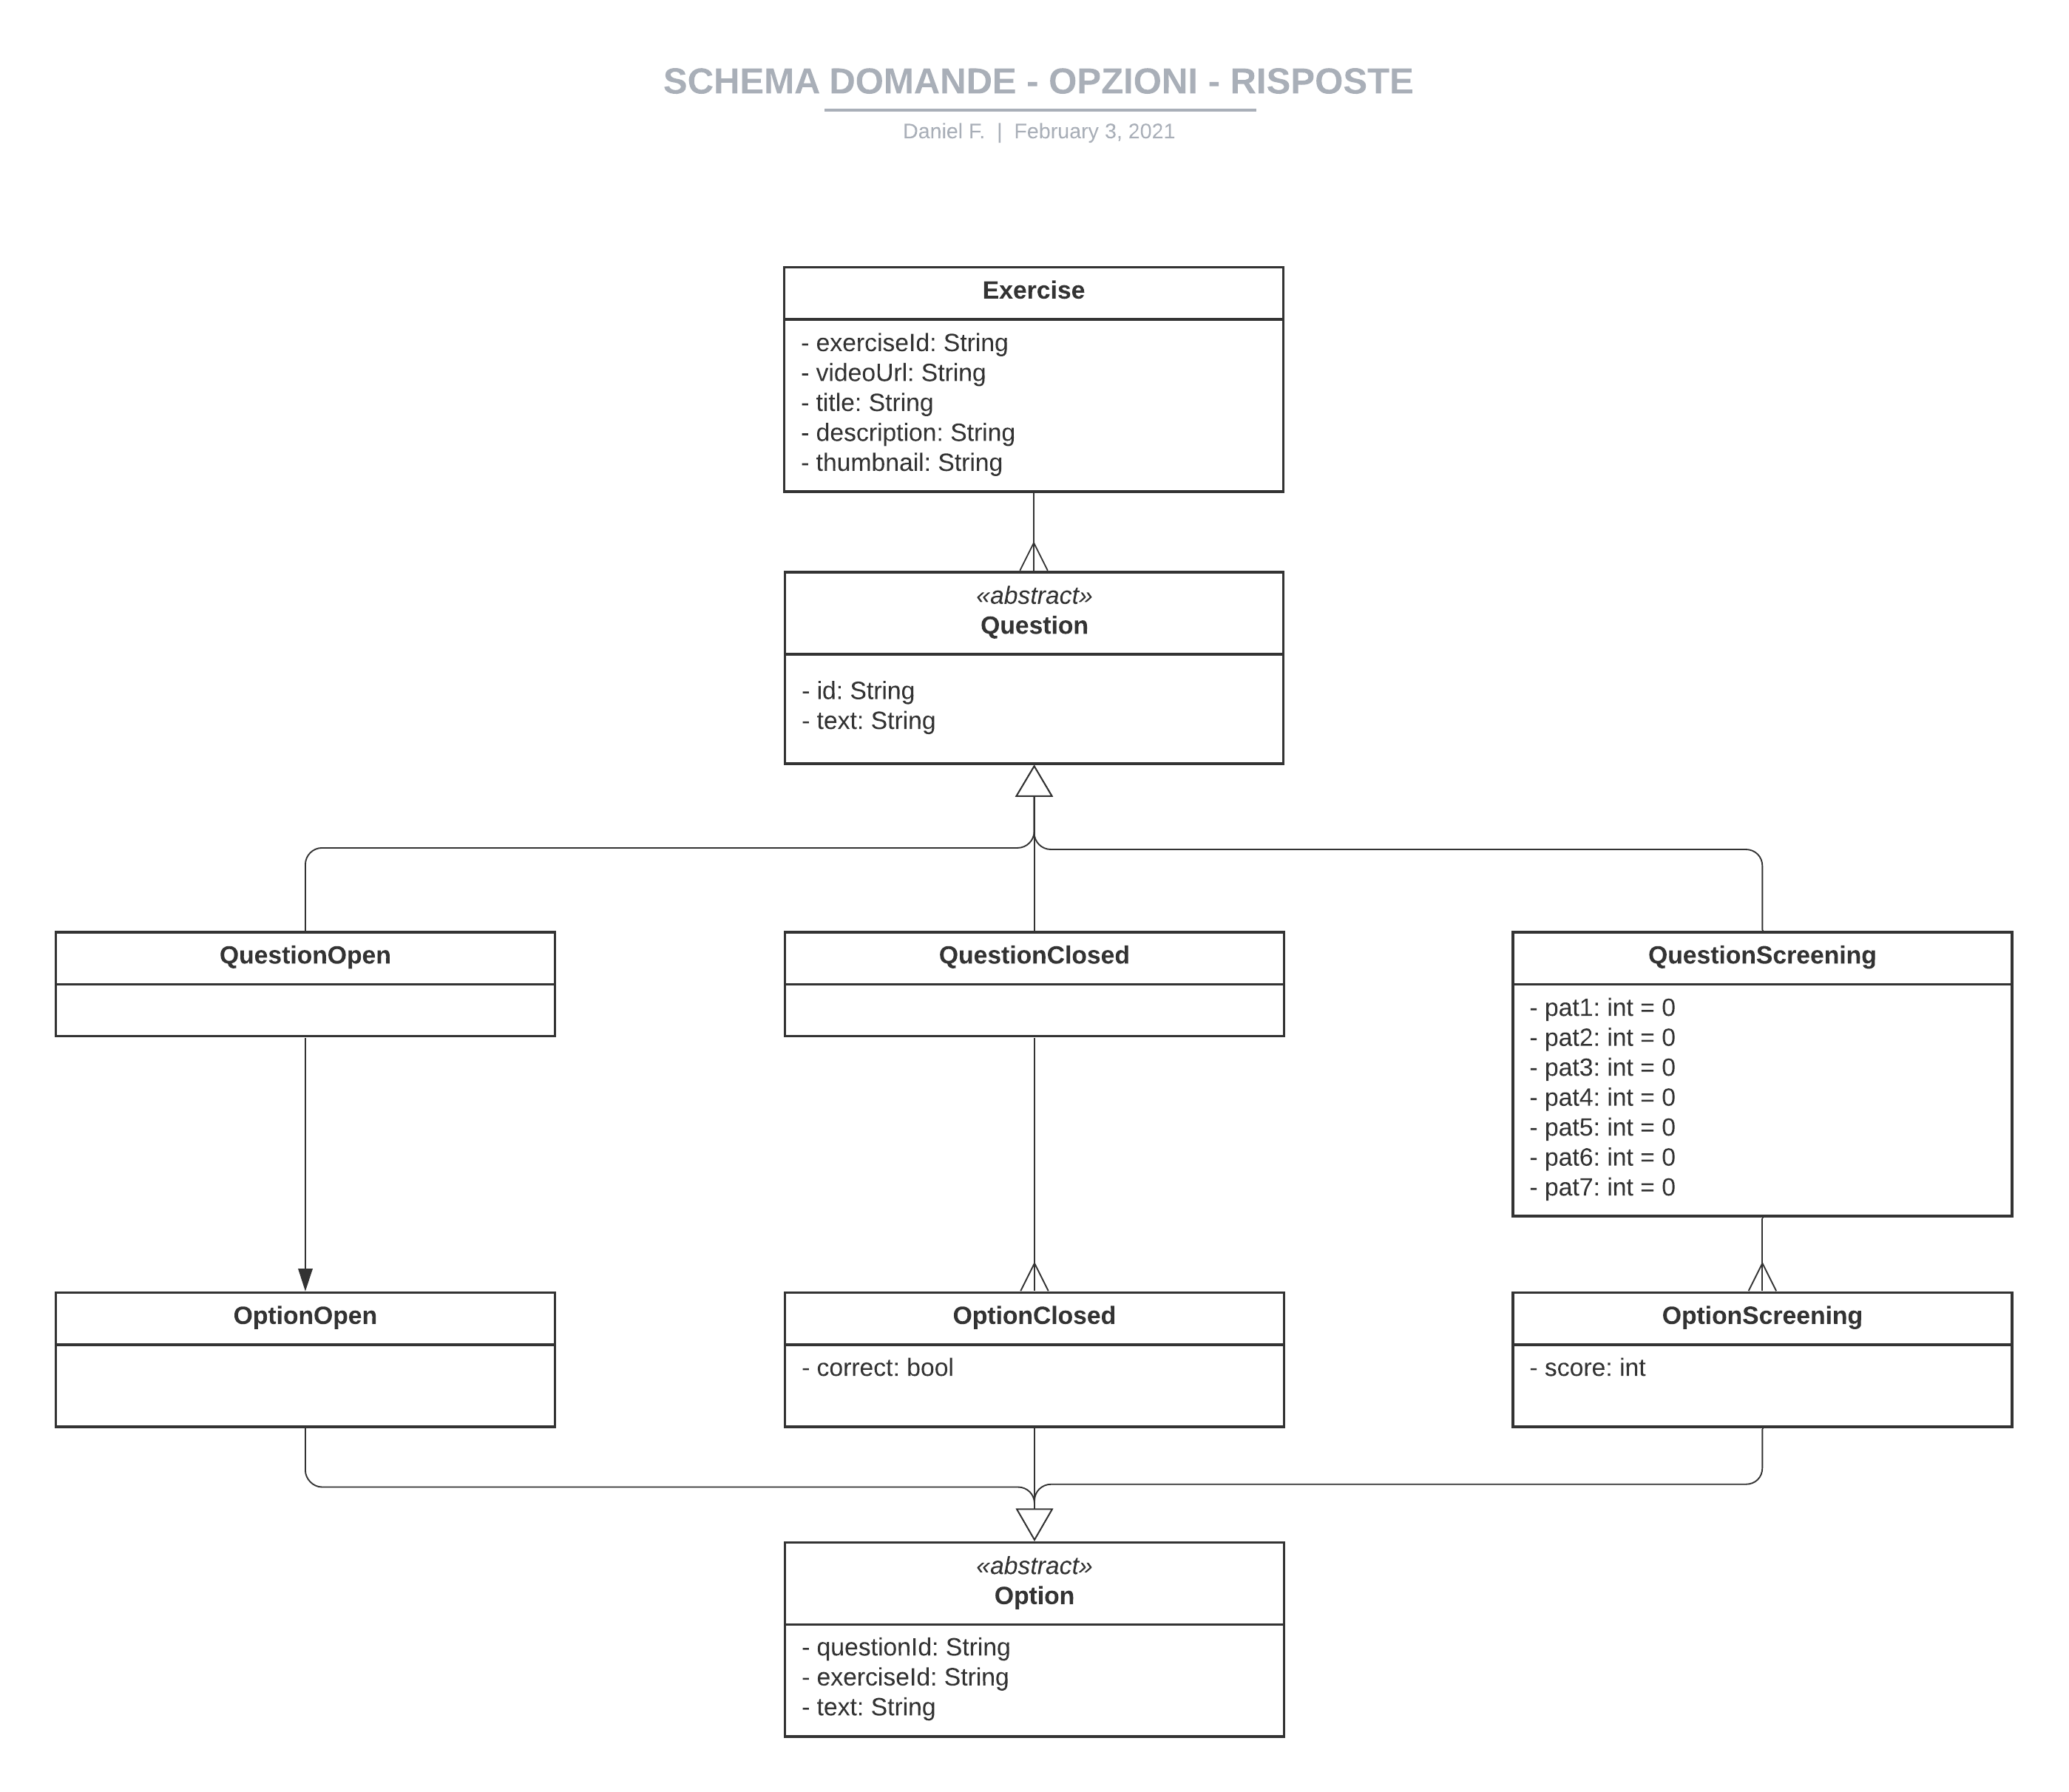
\includegraphics[width=\textwidth]{img/modello_iniziale}
\caption{Modello dati prima di Qualtrics}
\label{fig:modello_iniziale}
\end{figure}

\section{Dopo Qualtrics}
Non molto dopo i primi sviluppi è stato deciso di utilizzare \textbf{Qualtrics}\footnote{\url{www.qualtrics.com/uk/core-xm/survey-software}} come effettivo backend dell'applicazione, che non è altro che una piattaforma di creazione di sondaggi orientata alle aziende per ottenere feedback sia dai propri clienti che dai propri impiegati: l'idea era adattare questo software già pronto e che presenta già diversi tipi di domande utili al nostro scopo per poter ottenere gli input necessari dai nostri utenti e presentarli a chi di dovere. Non solo, essendo una piattaforma a sé stante, essa permette anche al gruppo di psicologia di creare i sondaggi necessari indipendentemente dallo sviluppo dell'applicazione, che si limita, tramite le API di Qualtrics, a ottenere e presentare questi sondaggi.

\subsection{Modello dati: domande}
In particolare, come possiamo vedere nel modello semplificato della Figura \ref{fig:modello_semplice_qualtrics}, il modello dati adottato da Qualtrics prevede un oggetto esterno, la \textbf{Survey} \textit{(sondaggio)}, che contiene, oltre a vari parametri di configurazione, una lista di \textbf{Questions} \textit{(domande, che sono degli oggetti anch'esse)} che possono essere di vario tipo; le domande a loro volta contengono i loro parametri di configurazione ed una lista di possibili risposte \textit{(Choices)} se a risposta chiusa.
Tra i valori interessanti contenuti nei parametri delle domande ci sono il \texttt{QuestionText}, che rappresenta la domanda vera e propria in linguaggio naturale, il \texttt{Selector} che permette di avere domande simili ma differenziate per qualche dettaglio \textit{(ad esempio possiamo avere una domanda a risposta chiusa in cui si possono selezionare più risposte piuttosto che solo una)} e il \texttt{ChoiceOrder}, che stabilisce in che ordine devono apparire le possibili risposte, contenute nell'oggetto \texttt{Choices}.
Ogni entità è inoltre opportunamente identificata, difatti le risposte non sono altro che delle coppie \texttt{<ID\_Domanda, ID\_Risposta>} oppure \texttt{<ID\_Domanda, [ID\_Risposta\_1, ..., ID\_Risposta\_n]>}, nel caso di domande a risposta chiusa, mentre nel caso di domande a risposta aperta sono del tipo \texttt{<ID\_Domanda, "Risposta">}.

\newpage

\subsection{Modello dati: blocchi}
Un aspetto particolare riguardo l'organizzazione delle domande nell'ambiente Qualtrics è quello legato ai \textbf{Blocks}, che sono degli insiemi di domande presentati separatamente. Questo permette di non sovraccaricare una schermata di domande ma di suddividerle in parti visualizzate indipendentemente.
Come si può vedere sempre nella Figura \ref{fig:modello_semplice_qualtrics}, i blocchi sono degli oggetti contenuti nell'oggetto \texttt{Survey} che dispongono di un \texttt{BlockID} e di una \texttt{Description}, una descrizione testuale utilizzata per dare un'idea del contesto delle domande presenti nel blocco. Inoltre, i blocchi contengono una lista di oggetti \texttt{BlockElements} che, seppur contente oggetti, non contiene le domande vere e proprie, ma solo gli \texttt{QuestionID} delle domande facenti parte del rispettivo blocco; è necessario quindi un incrocio dei dati nell'applicazione per far sì che le domande rispettino l'ordine dei blocchi.

È presente inoltre, sempre nell'oggetto\texttt{Survey}, un ulteriore oggetto \texttt{SurveyFlow} che contiene l'ordine di visualizzazione dei blocchi in una lista contenente i \texttt{BlockID} corrispondenti \textit{(in quanto potrebbero non essere nel giusto ordine all'interno dell'oggetto \texttt{Blocks})}.

\begin{figure}
\centering
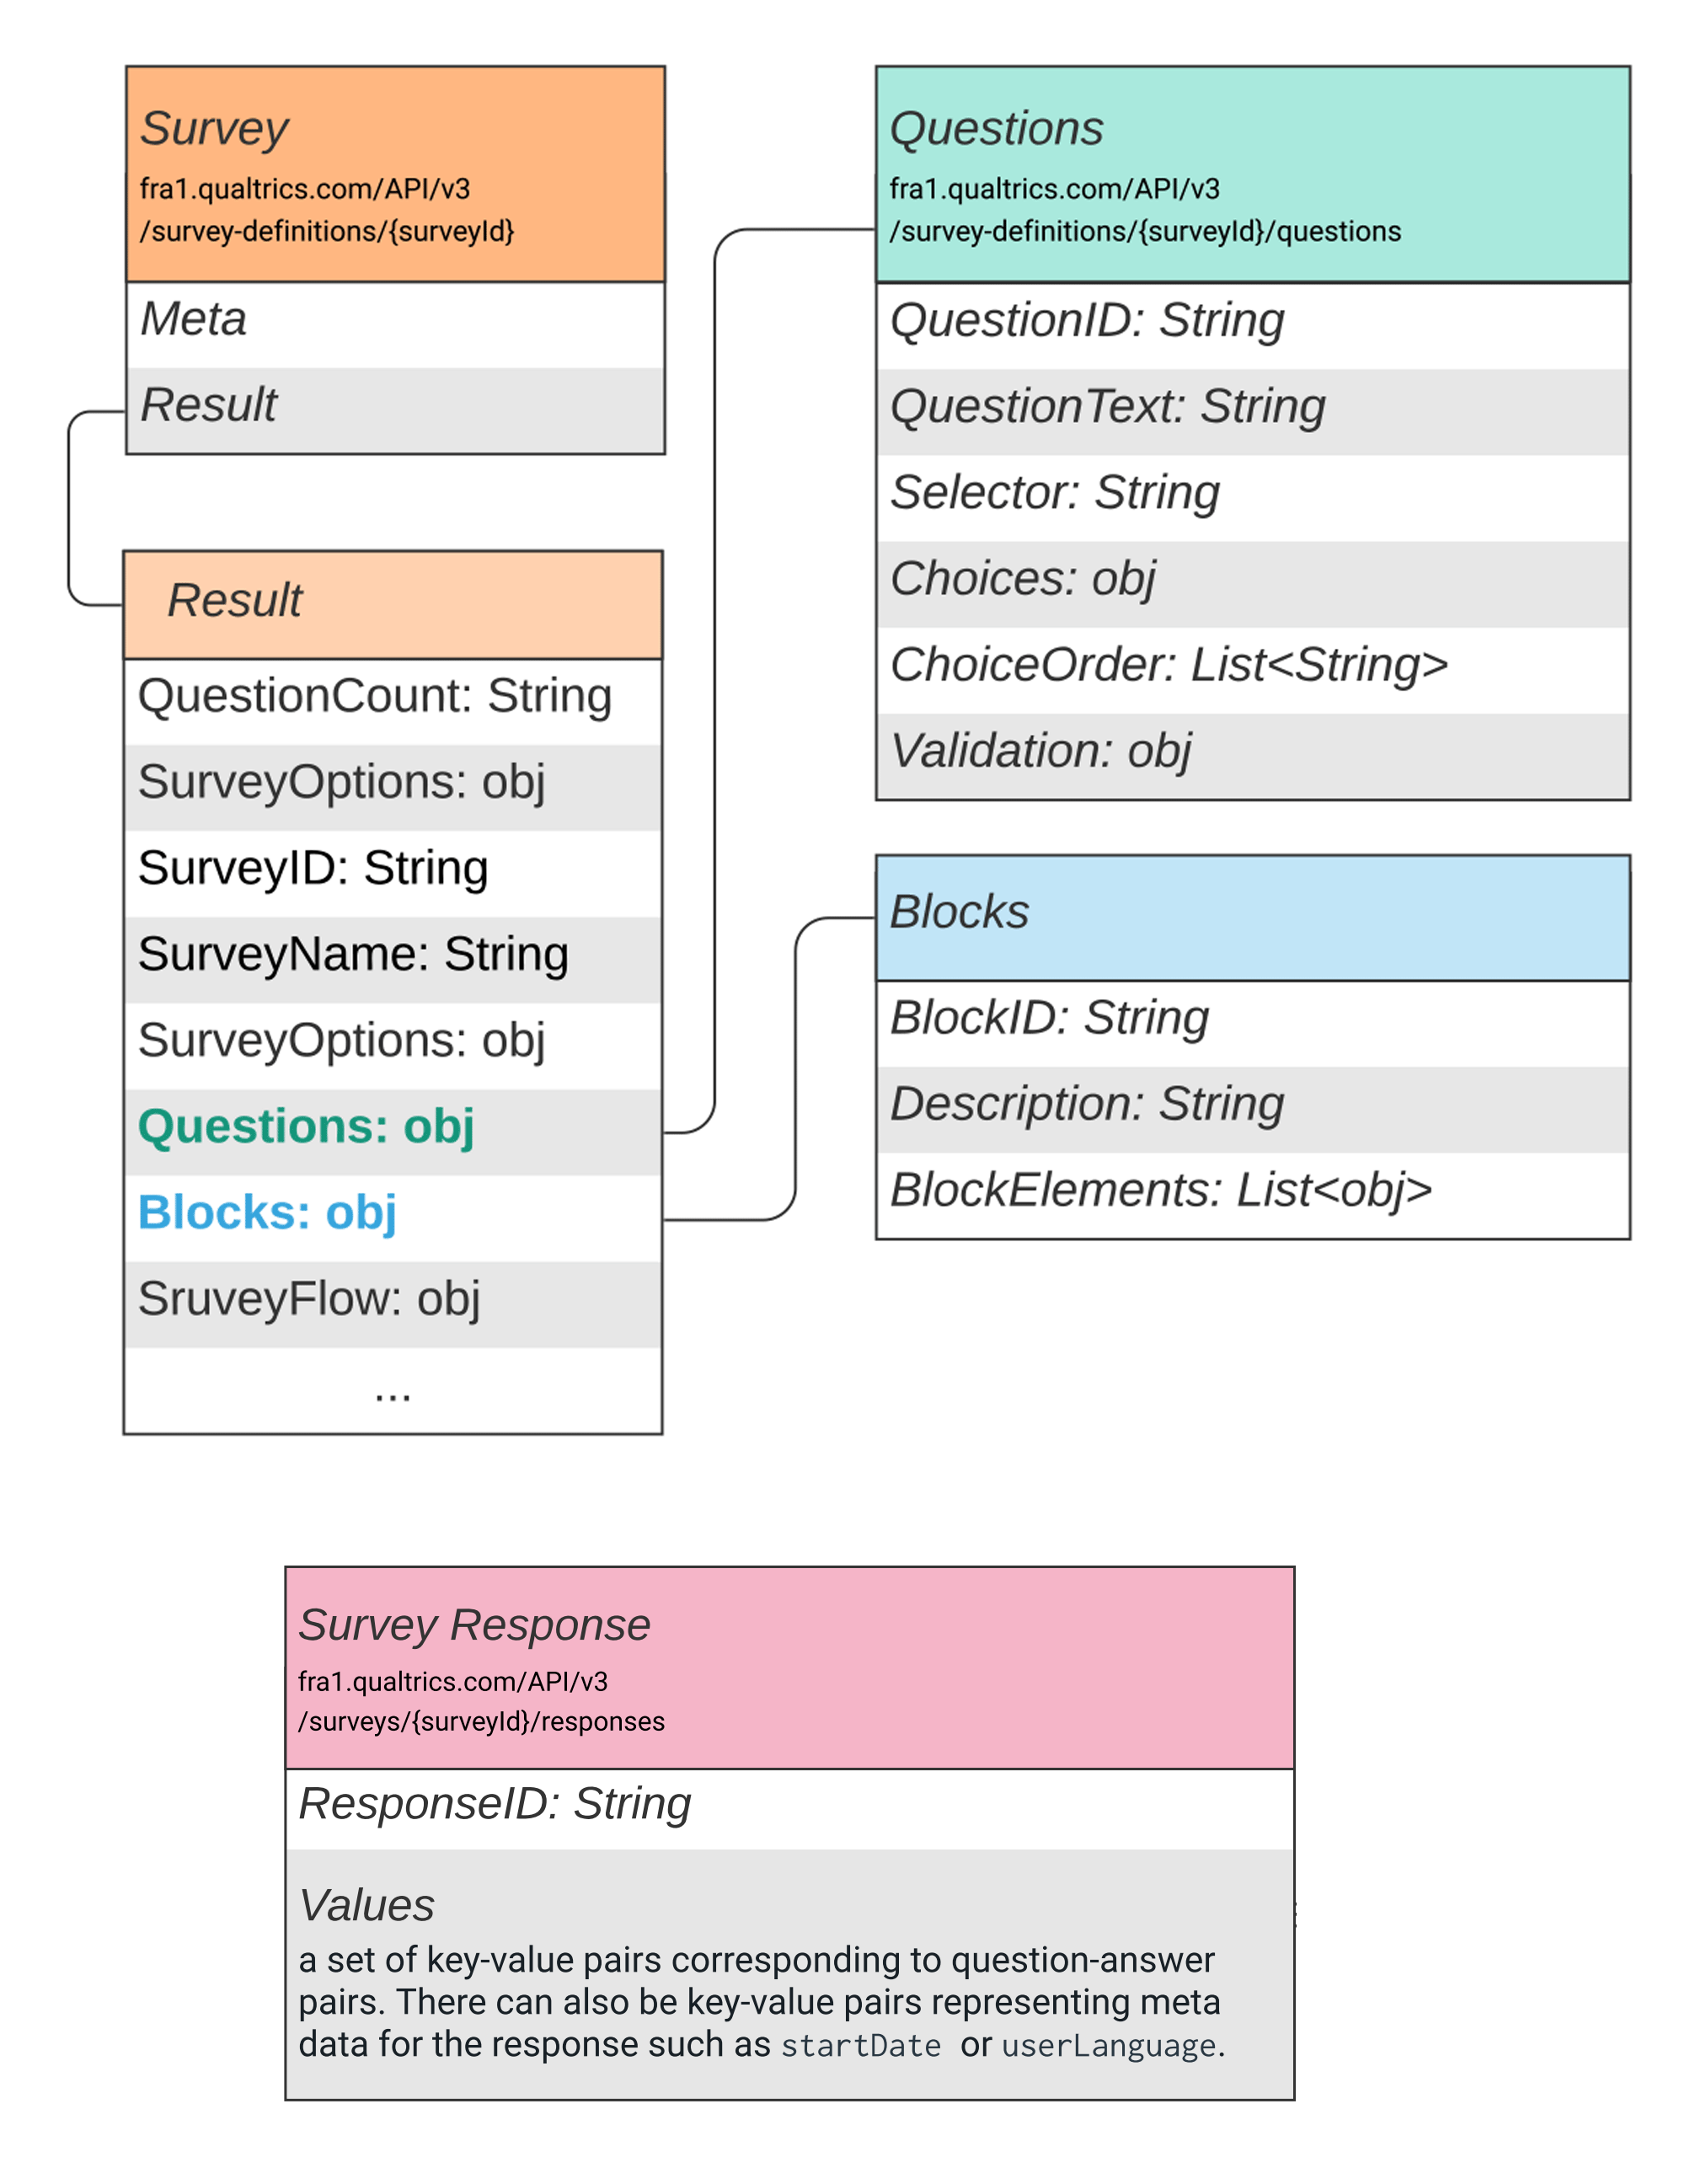
\includegraphics[width=\textwidth]{img/modello_semplice_qualtrics}
\caption{Modello dati Qualtrics semplificato}
\label{fig:modello_semplice_qualtrics}
\end{figure}